
ضخامت غشا از مرتبه‌ی چند نانومتر است و مقیاس انحنا‌هایی که شکل کلی غشا را مشخص می‌کنند از مرتبه‌ی بزرگی میکرون بوده. در نتیجه به طور عمومی مدل کردن شکل و انحنای غشا با یک رویه‌ی ۲ بعدی کاملا مورد قبول است. تصاویر میکروسکوپی غشا مانند شکل‌های 
\ref{fig:budding}
و
\ref{fig:flucmem} 
نشان می‌دهد که غشا سطحی نسبتا صاف و پیوسته دارد. در نتیجه در مقیاس‌های میکرومتری غشا را با رویه‌ای با چنین ویژگی‌ای مدل می‌کنیم. البته که این فرض در مقیاس نانومتری پابرجا نیست. 

\begin{figure}[h]
\begin{center}
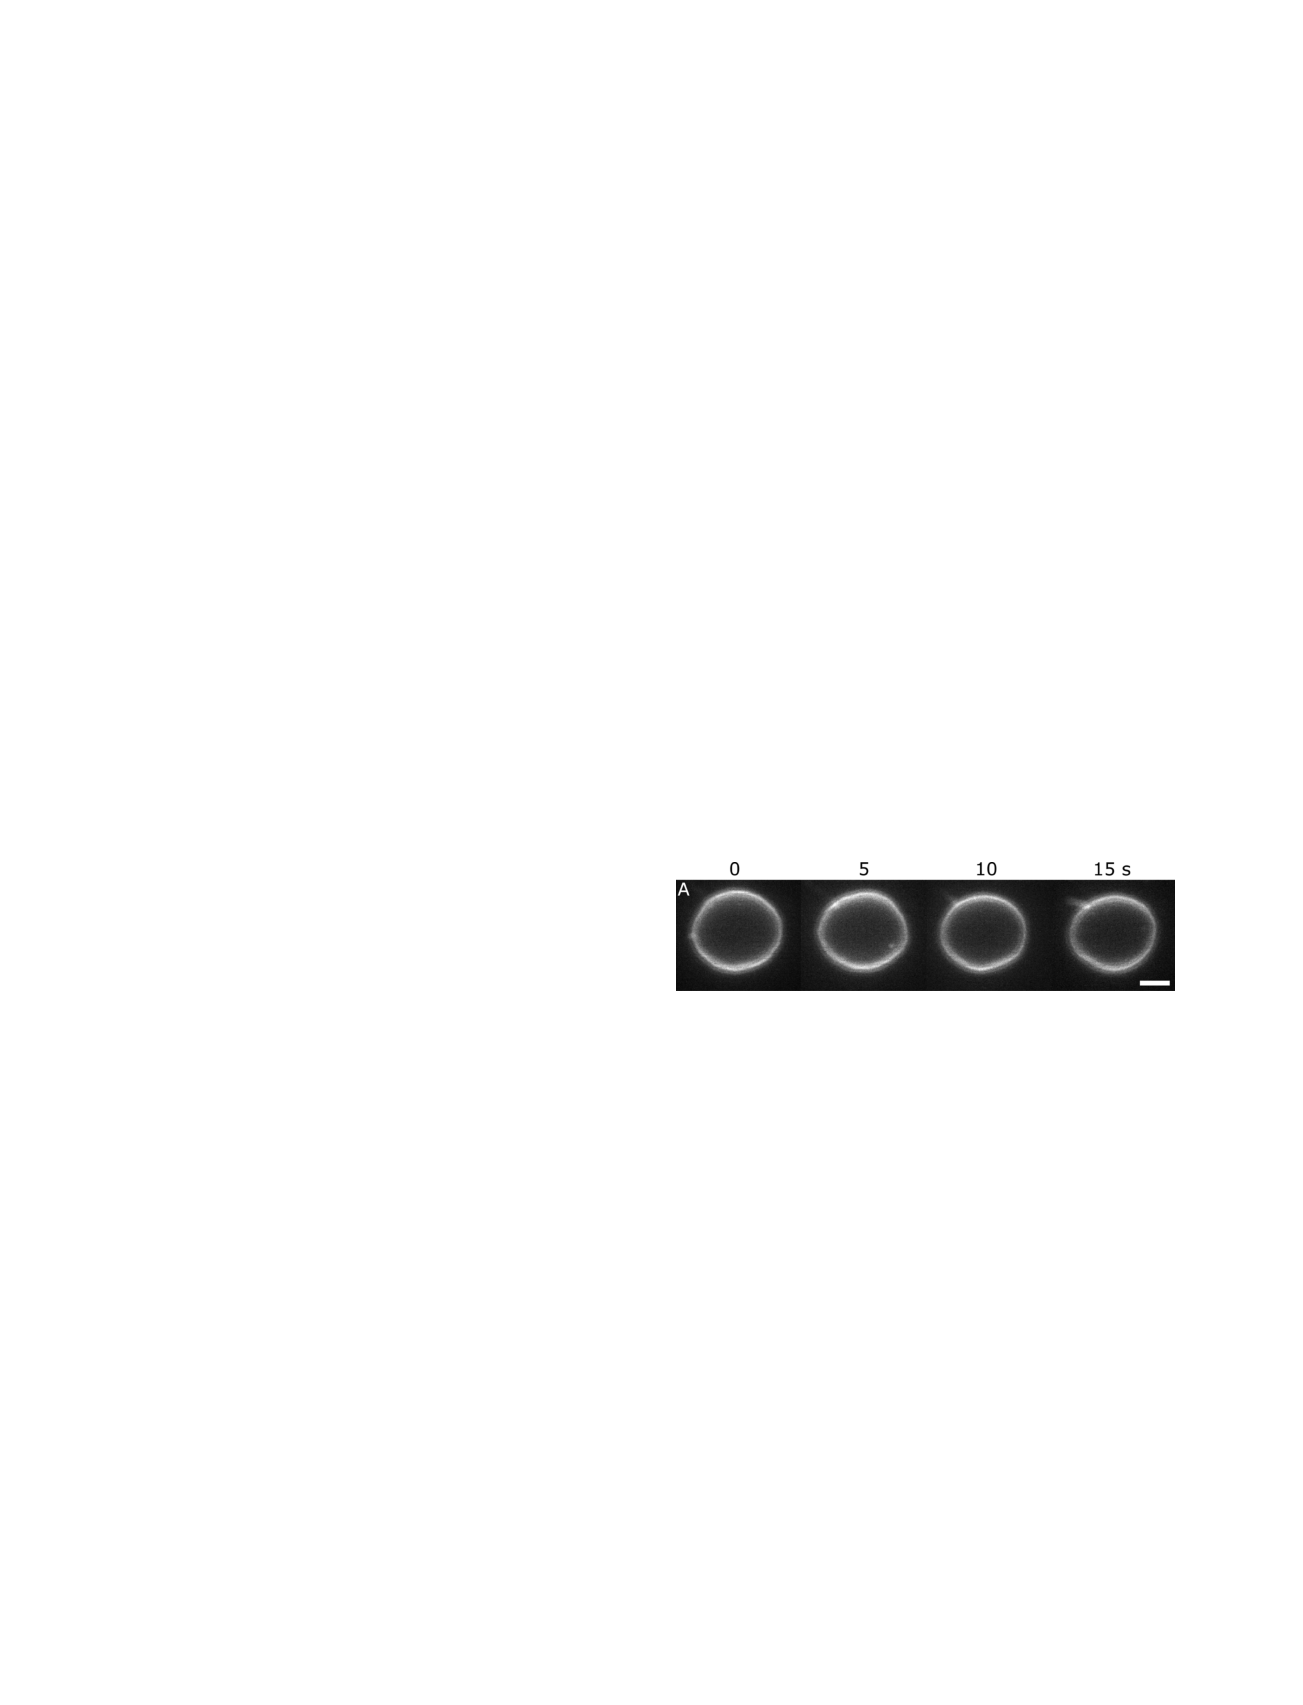
\includegraphics[width=6in]{\Mempath/Pics/Membrane_fluctuations}
\caption{
مجموعه تصاویر پست سر هم از تغییر شکل یک غشای لیپیدی را با تصویر برداری فلورسانت در بازه‌های ۵ ثانیه‌ای نشان می‌دهد. خط مقیاس سفید رنگ اندازه‌ی ۵ میکرومتر را نشان می‌دهد. 
\cite{ParthasarathyMembraneMeasurement}
}
\label{fig:flucmem}
\end{center}
\end{figure}

ملکول‌های غشا درون یک سیال غوطه‌ور است که تحت افت خیز ترمودینامیکی محیط در جهت‌ موازی سطح غشا و عمود بر آن در حال حرکت است. در نتیجه برای تعریف انحنا لازم است که سطح غشا به بخش‌های کوچک تقسیم بندی شود و با میانگین‌گیری رو  مکان ملکول‌ها انحنا را تغیین کرد. اندازه‌ی این بخش‌ها تابع شدت افت و خیز ملکول‌هاست. محاسبات حاصل از  شبیه‌ سازی دینامیک ملکلولی برای غشایی که ملکول‌های یکسان داد حدود ۱.۵ برابر ضخامت غشا گزارش شده است
\cite{Goetz1998}
. از آنجایی که برای یک غشای ساده با ضخامت 
$4nm$
خمش هر بخش حاصل از رفتار دست جمعی حدود 
$100$
ملکول لیپیدی خواهد بود. در مقیاس بزرگ هر کدام از این بخش‌ها یک نقطه بر روی رویه‌ی غشا هستند. ما می‌توانیم برای هر نقطه روی غشا یک صغحه‌ی مماس و یک صفحه‌ی عمود بر مماس تعریف کنیم. صفحه‌ی عمود بر سطح با رویه‌ی غشا فصل مشترکی به شکر یک خط دارد.  (مانند شکل 
\ref{fig:normalPlaneIntersection}
).
\begin{figure}[h]
\begin{center}
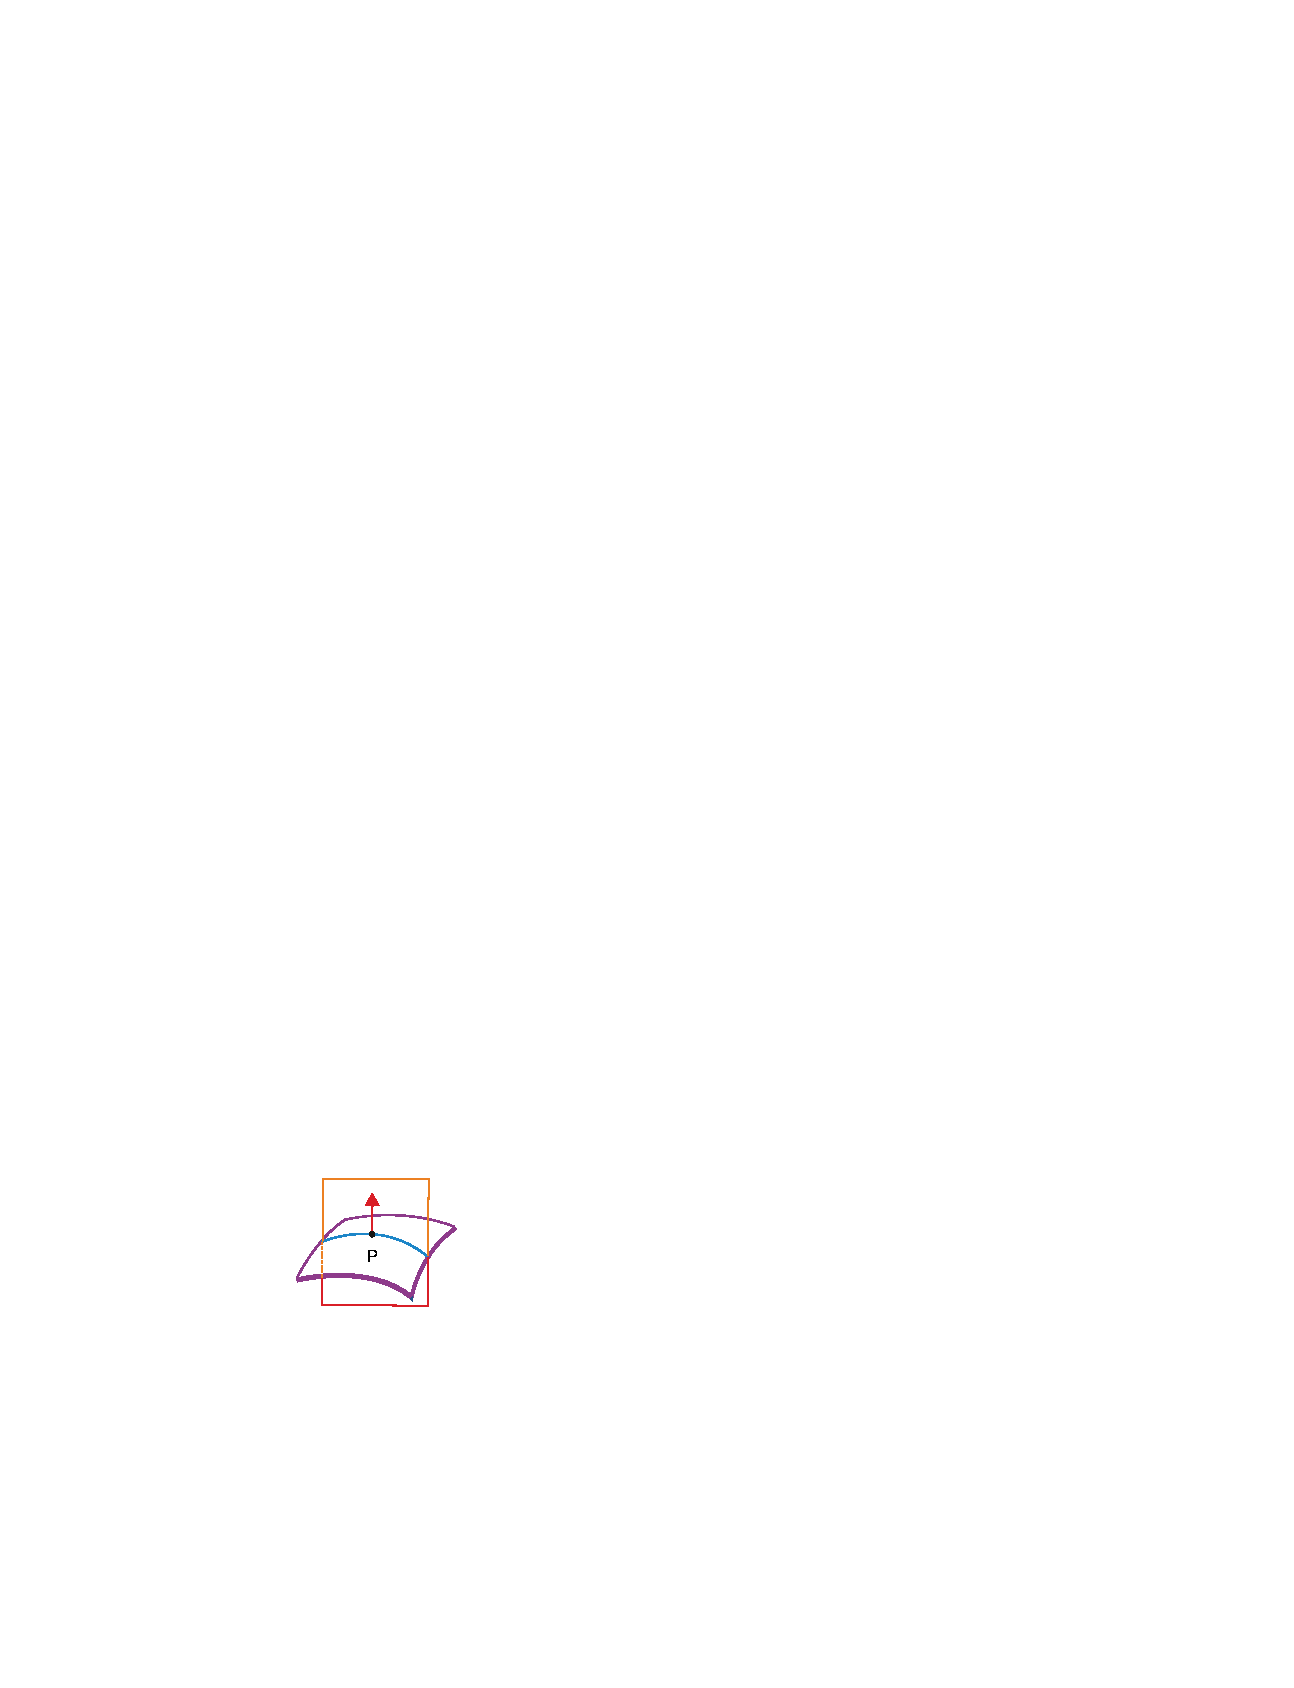
\includegraphics[width=6in]{\MemTB/Pics/NormalPlane}
\caption{
خم حاصل از فصل مشترک صفحه‌ی عمود بر سطح غشا در نقطه‌ی 
P
را نشان می‌دهد.
}
\label{fig:normalPlaneIntersection}
\end{center}
\end{figure}
برای خم تشکیل شده از فصل مشترک می‌توان خمش
$C$
تعریف کرد به صورتی که اگر انحنا در جهت بردار عمود بر سطح باشد (
$\cap$
) آنرا با علامت مثبت و در حالتی که در جهت مخالف باشد (
$\cup$
) آنرا با علامت منفی نشان می‌دهیم. می‌توان فرض کرد که خط مشترک قسمتی از یک دایره  است و خمش این خط عکس شعاع دایره خواهد بود. یک انتخاب برای صفحه‌ی مماس بر سطح وجود ندارد ولی صفحه‌ی عمود بر سطح می‌تواند در جهت‌های مختلف تعریف شود که خمش‌های مختلفی را تعریف کند. اگر تمام خمش‌های ممکن در یک نقطه‌ را با تغییر جهت صفحه‌ی متعامد اندازه‌گیری کنیم، اندازه‌گیری ما در یک بازه‌ای محدود به مقادیر کمینه و بیشینه‌ی خمش در آن نقطه قرار خواهد گرفت،
$C_{min}$
و
$C_{max}$
. مقادیر کمینه و بیشینه خمش به خمش‌های اصلی سطح معرف هستند که با 
$C_1$
و
$C_2$
نمایش داده می‌شوند. خمش‌های اصلی همچنین  ویژه‌مقدار‌های تانسور خمش در آن نقطه هستند. همچنین اگر خمش‌های اصلی برابر یکدیگر نباشند،
$C_1\neq C_2$ 
صفحاتی که خم‌ها با آن تعریف می‌شوند حتما عمود بر هم خواهند بود. از آنجایی که ملکول‌های سطح غشا حرکت پخشی می‌کنند  شکل غشا باید بر اساس تعاریفی باشد که تحت تغییر روش پارامتریزه
\LTRfootnote{paprameterisation}  
 کردن سطح ناوردا باشد. خمش‌های اصلی سطح چنین ویژگی دارند. خمش میانگین در هر نقطه‌ بر روی سطح به صورت 
\begin{equation}
M=\frac{1}{2}(C_1+C_2)
\label{eq:meanCurv}
\end{equation}
و خمش گاووسی به صورت
\begin{equation}
G=C_1C_2
\label{eq:gaussianCurv}
\end{equation}
 تعریف کرد. خمش میانگین معادل رَد
\LTRfootnote{trace} 
 تانسور خمش و خمش گاووسی برابر با دترمینان این تانسور است. همچنین می‌توان روابط بالا را بازنویسی کرد و خمش‌های اصلی را بر حسب خمش میانگین و خمش گاووسی محاسبه کرد،

\begin{figure}[h]
\begin{center}
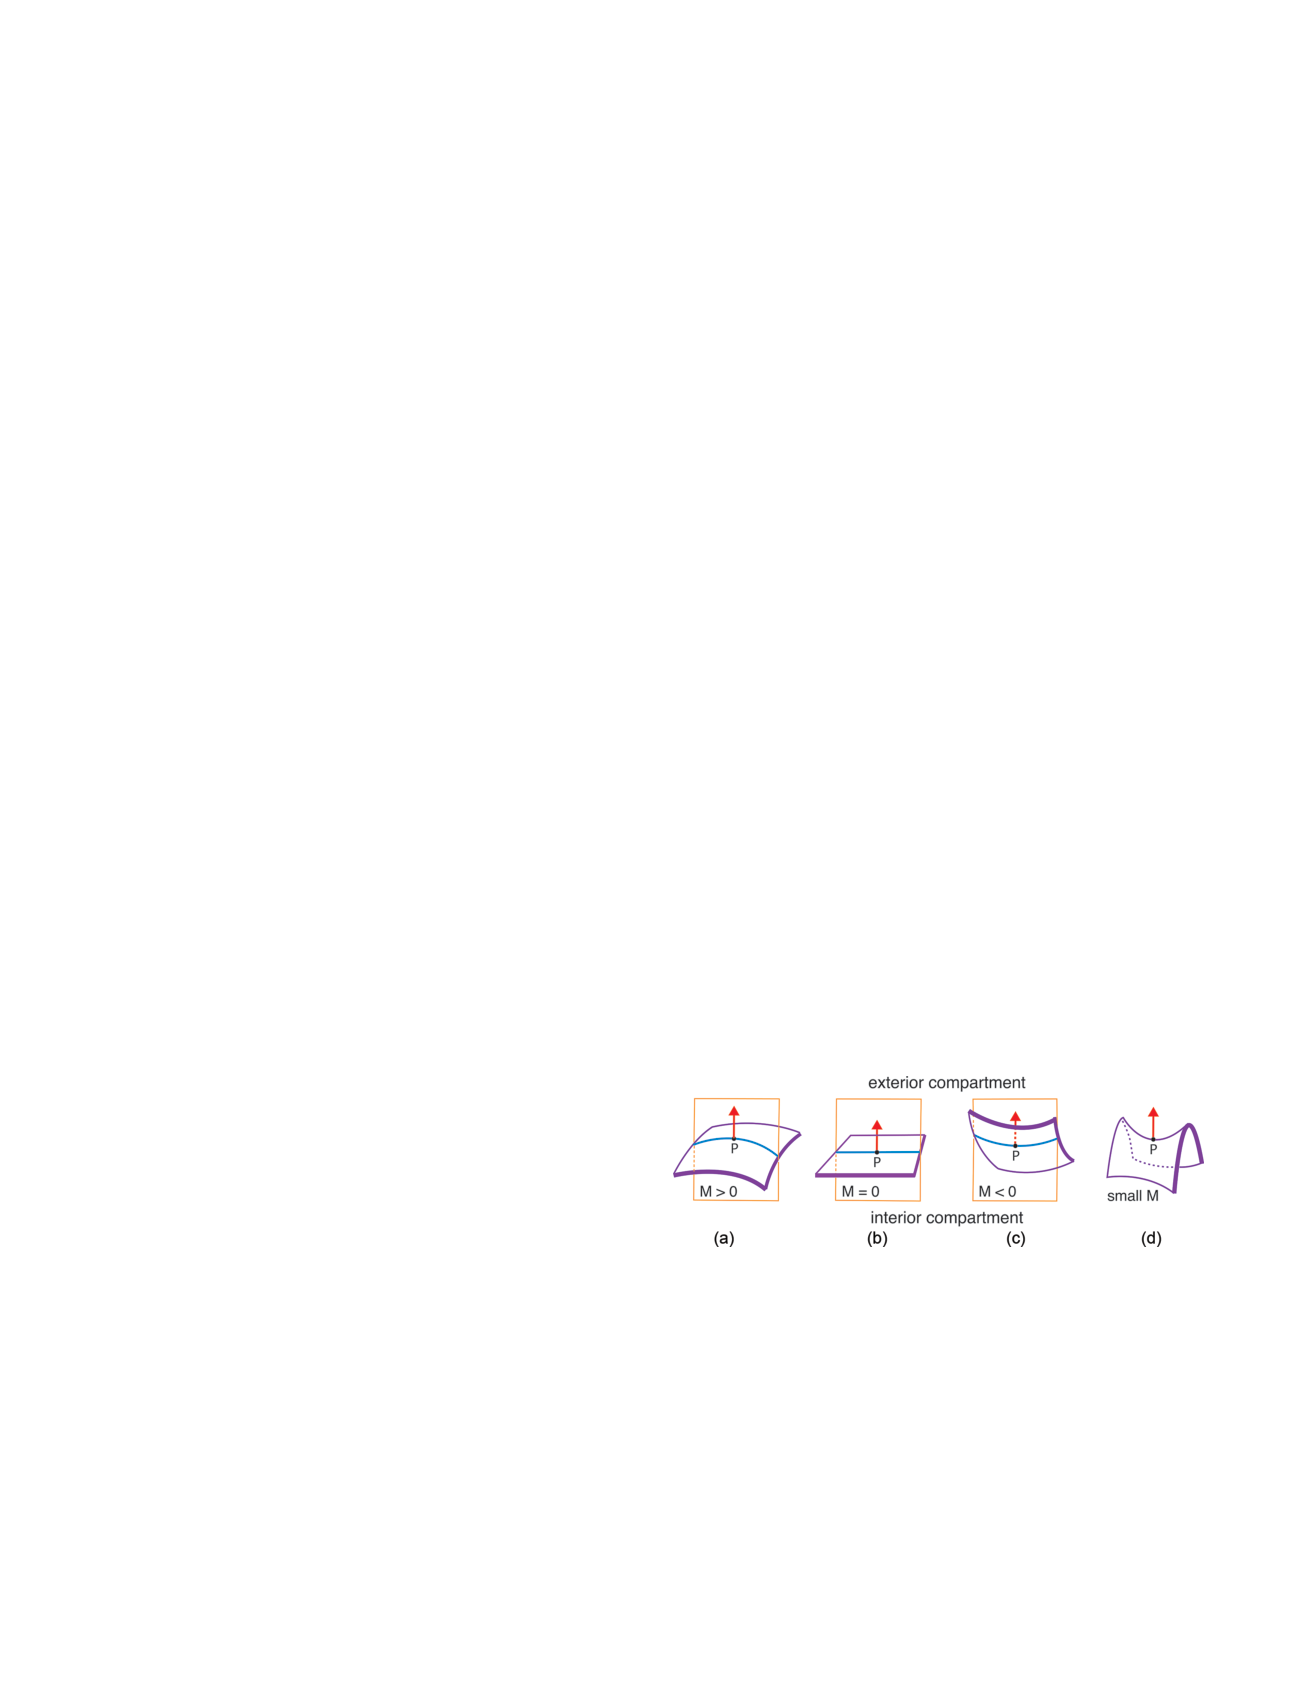
\includegraphics[width=6in]{\MemTB/Pics/curvatureSign}
\caption{
قرارداد برای تعیین علامت خمش میانگین. با فرض اینکه بالا محیط خارج غشا و پایین داخل غشا را مشخص کند، بردار نرمال غشا جهت (بردار قرمز رنگ) رو به بالا خواهد داشت. در شکل الف) خمش میانگین مثبت هنگامی که هر دو خمش اصلی برآمدگی در جهت بردار نرمال داشته باشند. ب) برای قسمت تخت خمش میانگین صفر، ج) خمش منفی هنگامی که  برآمدگی به سمت داخل غشا باشد، د) در نقاط زین اسبی خمش‌های اصلی علامت‌های مخالف یکدیگر دارند و در این صورت خمش میانگین مقدار کمی خواهد داشت.
}
\label{fig:curvatureSign}
\end{center}
\end{figure}

\begin{equation}
\begin{aligned}
C_1&=M-\sqrt{M^2-G}\\
C_2&=M+\sqrt{M^2-G}.
\label{eq:gaussianCurv}
\end{aligned}
\end{equation}
که در روابط بالا، از آنجایی که 
$M^2\geq G$
\cite{Seifert1991}
 هر دو مقدار همیشه حقیقی هستند. مقدار خمش میانگین، 
 $M$،
 تحت تمامی تبدیل‌های دستگاه مختصات که دترمینان ژاکوبین آن مثبت باشد (جهت بردار عمود بر سطح را تغییر ندهد) تغییر نخواهد کرد. به طور مثال اگر یک سطح با پارامتر‌های 
 $(s^1,s^2)$
 تعریف شده باشد، تبدیلی که پارامتر‌ها را با یکدیگر تعویض کند، 
 $(s^{-1}\equiv s^2,s^{-2}\equiv s^1)$
 تبدیلی است که جهت نرمال سطح را تغییر می‌دهد که در نتیجه علامت خمش میانگین را تغییر می‌دهد. هرچند که چنین تبدیل‌هایی در فیزیک بسیار مهم هستند زیرا که انتخاب دستگاه مختصات بر مشخصات برخی خواص فیزیکی نباید تاثیرگذار باشد، ولی در مورد خمش باید تعریف مشخصی برای محاسبات وجود داشته باشد تا بتوان میان محیط داخل و خارج غشا تمییز قائل بشویم. با توجه به رابطه‌ی
 \ref{eq:meanCurvature}
 علامت خمش میانگین در هر نقطه روی غشا تابع مقادیر خمش‌های اصلی در آن نقطه‌ است. شکل 
 \ref{fig:curvatureSign}
 حالت‌های مختلف که بر علامت خمش میانگین تاثیر می‌گذارد را نشان می‌دهد. 

به طور کلی، برای سطح تخت خمش میانگین صفر است، در صورتی که برآمدگی خمش به سمت داخل غشا باشد، خمش میانگین منفی و در صورتی که برآمدگی به سمت بیرون غشا باشد، خمش میانگین مثبت خواهد بود. در نقاط زین اسبی خمش‌های اصلی علامت‌های مخالف یکدیگر دارند و در نتیجه مقدار خمش میانگین بسیار کوچک خواهد بود. مهم است که اشاره شود که خمش میانگین ابزار مناسبی برای اندازه‌گیری تاثیر نقاط زین اسبی نیست زیراکه مقدار آن با سطح تخت اختلاف چندانی ندارد. برای اندازه‌گیری تاثیر نقاط زین اسبی، خمش گاووسی ابزار مناسبی است.
\begin{figure}[h]
\begin{center}
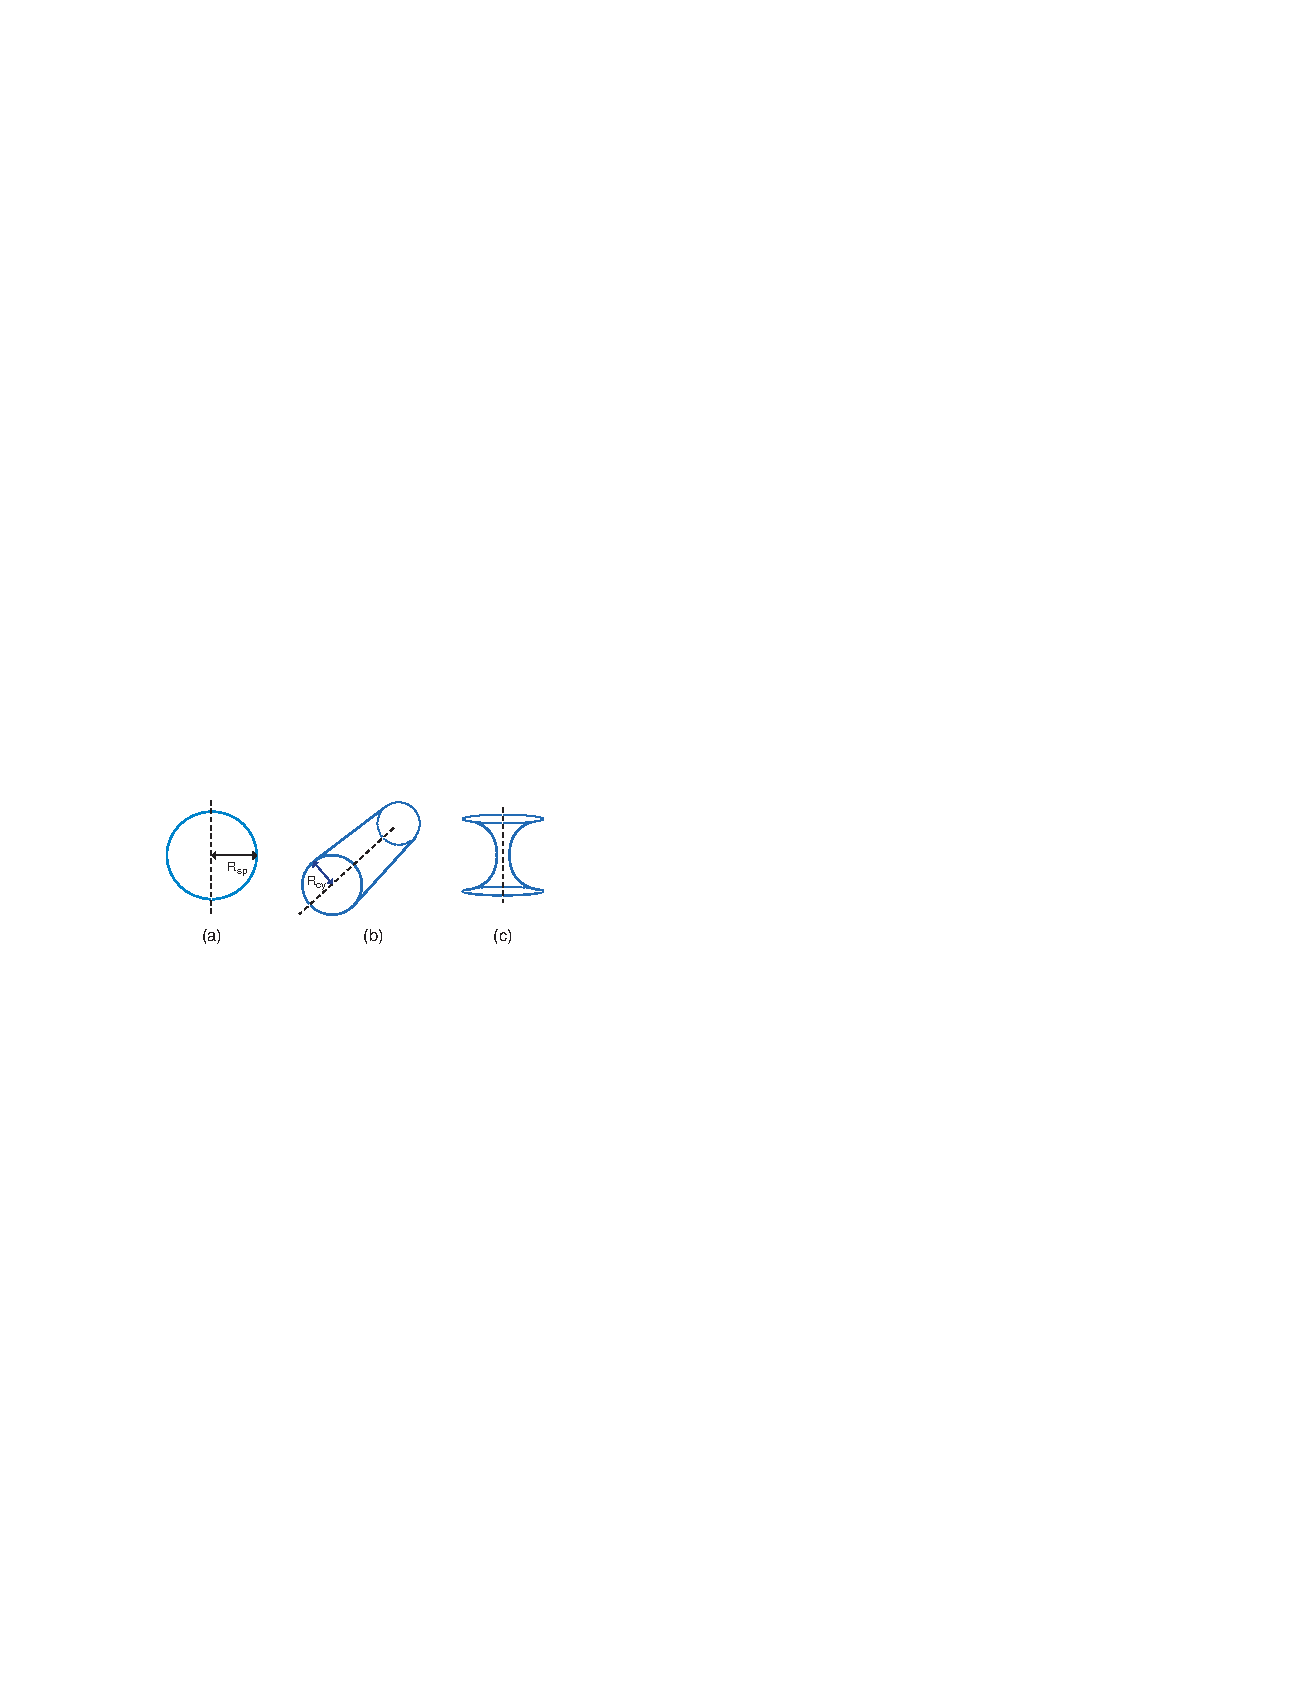
\includegraphics[width=6in]{\MemTB/Pics/simpleMembraneShapes}
\caption{
شکل‌های ساده‌ی غشا که در تمام نقاط روی سطح خمش میانگین ثابتی دارند. شکل الف، کُره‌ای به شعاع 
$R_{sp}$
با خمش میانگین 
$M=\pm 1/R_{sp}$
ب، استوانه‌ای با شعاع 
$R_{cy}$
با خمش میانگین
$M=\pm 1/2R_{cy}$
و در نهایت ج، کتانوید با خمش میان صفر. علامت خمش میانگین برای کُره و استوانه به این بستگی دارد که محیط بیرون، سیال خارج از غشا تعریف شود یا سیال داخل.
}
\label{fig:simpleMembraneShapes}
\end{center}
\end{figure}
به طور عمومی خمش میانگین یک کمیت موضعی است و در نقاط مختلف روی سطح غشا تغییر می‌کند. اما برخی اَشکال ساده در تمامی نقاط روی سطح خود یک مقدار ثابت خمش میان‌گین دارند. برای مثال خمش میانگین یک غشای تخت صفر است. برای مثال‌های بیشتر با شکل 
\ref{fig:simpleMembraneShapes}
توجه کنید. خمش میانگین یک کُره با شعاع
$R_{sp}$
برابر با 
$C=1/R_{sp}$
هنگامی که لایه‌ی خارجی آن با محیط بیرون غشا در ارتباط است و 
$C=-1/R_{sp}$
زمانی که لایه‌ی داخلی آن با محیط بیرون در ارتباط است. همچنین استوانه‌‌ای با شعاع 
$R_{cy}$
دارای خمش میانگین
$C=\pm1/2R_{cy}$
که علامت آن تابع تعریف جهت بردار عمود خواهد بود. یک شکل ساده‌ی جالب، کتانوید
\LTRfootnote{catanoid} 
 است که تمام نقاط روی سطح آن از نقاط زین اسبی تشکیل شده و در نتیجه خمش میانگین همه جا خمش میانگین آن صفر است.





 
 
 
 
 


